% LaTex document
%\pagelayout{normal}
%\input epsf

\documentclass[11pt]{article}
\usepackage{rotating}
%\usepackage{epsfig}
\usepackage{color}
\usepackage{graphicx}
\usepackage{xspace}
\usepackage{lineno}
%\usepackage{feynmp}
\topmargin -0.5in
\oddsidemargin 0in
\evensidemargin 0in
\textheight 8.9in
\textwidth 6.50in
\parskip 3pt plus 1pt minus 0.5pt
\newlength{\COTlength}
\setlength{\COTlength}{2.5pt plus 8pt minus 0pt}


\graphicspath{/Users/samantha/apsnote/PDFS/}

%insert line number for proof reading. comment out these when making the final pdf
\linenumbers
\leftlinenumbers*

\begin{document}
\begin{flushright}
CDF/ANAL/EXOTIC/CDFR/9267 \\
Version 0.3 \\
%\rm \today
\vspace*{-0.2truein}
\end{flushright}

\def\sla#1{\rlap{\kern .15em /}#1}

\newcommand{\w}{\mbox{$W$}\xspace}
\newcommand{\z}{\mbox{$Z$}\xspace}
\newcommand{\zee}{\mbox{$Z\rightarrow e^+e^-$}\xspace}
\newcommand{\zmm}{\mbox{$Z\rightarrow \mu^+\mu^-$}\xspace}
\newcommand{\ztt}{\mbox{$Z\rightarrow \tau^+\tau^-$}\xspace}
\newcommand{\wen}{\mbox{$W\rightarrow e+\nu$}\xspace}
\newcommand{\wmn}{\mbox{$W\rightarrow \mu+\nu$}\xspace}
\newcommand{\wtn}{\mbox{$W\rightarrow \tau+\nu$}\xspace}

\newcommand{\zgee}{\mbox{$Z/\gamma^*\rightarrow e^+e^-$}\xspace}
\newcommand{\W}{\mbox{$W^\pm$}\xspace}
\newcommand{\Wenu}{\mbox{$W^\pm\rightarrow e^\pm\nu$}\xspace}
\newcommand{\wenu}{\mbox{$W\rightarrow e\nu$}\xspace}
\newcommand{\wmnu}{\mbox{$W\rightarrow \mu\nu$}\xspace}
\newcommand{\wtnu}{\mbox{$W\rightarrow \tau\nu$}\xspace}

\newcommand{\pt}{\mbox{$p_T$}\xspace}
\newcommand{\et}{\mbox{$E_T$}\xspace}
\newcommand{\etcorr}{\mbox{$E_T^{corr}$}\xspace}
\newcommand{\ecorr}{\mbox{$E^{corr}$}\xspace}
\newcommand{\met}{\mbox{$\sla{E}_T$}\xspace}
\newcommand{\eoverp}{\mbox{$E/p$}\xspace}
\newcommand{\isoetcorr}{\mbox {$E_ {T}^{Iso(corr)}$\xspace }}
%\newcommand{\gammajets}{\mbox{$\gamma$  + $\gt\eq$1~jets + $\met$}}
%text formatting
\newcommand{\superscript}[1]{\ensuremath{^\textrm{#1}}}
\newcommand{\subscript}[1]{\ensuremath{_\textrm{#1}}}
%\newcommand{\th}[0]{\superscript{th}}
%\newcommand{\st}[0]{\superscript{st}}
%\newcommand{\nd}[0]{\superscript{nd}}
%\newcommand{\rd}[0]{\superscript{rd}}
%\newcommand{\halojets}{\mbox{{$\gammma^{Halo}~+~jets$}\xspace}}
\newcommand{\phojets}{\mbox{$\gamma$ + jets}\xspace}
\newcommand{\phoonejet}{\mbox{$\gamma +\geq $1 jet}\xspace}
\newcommand{\photwojet}{\mbox{$\gamma +\geq $2 jets}\xspace}
\newcommand{\phojetsmet}{\mbox{\phojets + \met}\xspace}
\newcommand{\elejets}{\mbox{$\gamma^{e\rightarrow\gamma}$ + jets}\xspace}
\newcommand{\cosmicjets}{\mbox{$\gamma^{cosmic}$ + jets}\xspace}
\newcommand{\halojets}{\mbox{$\gamma^{halo}$ + jets}\xspace}
\newcommand{\pbi}{\mbox{pb$^{-1}$}\xspace}
\newcommand{\pho}{\mbox{$\gamma$}\xspace}
\newcommand{\intimewindow}{\mbox{$-4.8$~ns $< t <$ +4.8~ns}\xspace}
\newcommand{\cosmictimewindow}{\mbox{+30~ns $< t <$ +90~ns}\xspace}
\newcommand{\etg}[1]{\mbox{$\et >$ #1~GeV}\xspace}
\newcommand{\timewindow}[2]{\mbox{$#1$~ns$~< t <#2$~ns}\xspace}

\title{Search for Anomalous Production of Photon + Jets + \met}
\author{Samantha Hewamanage, Jay Dittmann, Nils Krumnack\\
    {\it Baylor University} \\
    \\
Raymond Culbertson, Sasha Pronko \\
    {\it Fermilab} \\
}

\def\newpage{\par\penalty 100}          % hack \newpage
\maketitle
\def\newpage{\par\vfill\penalty -10000} % restore

\vspace*{-0.1truein}
\def\newpage{\par\penalty 100}          % hack \newpage

\begin{abstract}
\noindent 
Many new physics models predict mechanisms that could produce a $\gamma$ and jets signature.  We search in the $\gamma$ + jets and \phojetsmet channels, independent of any model, for new physics using 2~fb$^{-1}$  of CDF Run II data collected at the Fermilab Tevatron from $p\bar{p}$ collisions at $\sqrt{s} = 1.96$ TeV. A variety of techniques are applied to estimate the standard model expectation and non-collision backgrounds. We examine several kinematic distributions including \met, $\Sigma \et$, and invariant masses for discrepancies with the standard model. 
\end{abstract}

\pagestyle{plain}


\section{Introduction}
We present the preliminary findings of  \phojetsmet signature-based search. We begin by describing the datasets used in this analysis. Then we explain the signal selection, sources of backgrounds, and the methods used to estimate the remaining backgrounds in the signal sample. 

\section{Datasets}
We use the high-\pt photon datasets \texttt{cph10d}, \texttt{cph10h}, \texttt{cph10i}, and \texttt{cph10j} which were collected at CDF during the run periods 1--13 (run range 190851 to 246231) with triggers \mbox{PHOTON\_ISO\_25}, \mbox{PHOTON\_50}, and \mbox{PHOTON\_70}. These triggers are high-\pt photon triggers which suit our resonance search.  Good run list \texttt{goodrun\_v19\_pho\_00} from the Photon Group is used to estimate the luminosity.  After the good run selection the total luminosity is  2043~\pbi and this is excludes the first 400~\pbi of data (run range $>=$138425 \& $<$190851) that has no EM timing information.

We use Monte Carlo data samples for validation, cross checks, and to predict the shape of the electroweak background and fake \met from real $\gamma$ events. 

\begin{enumerate}
 \item{Inclusive $\gamma$ dataset \texttt{jqcdfh} \textsc{Pythia} Monte Carlo sample generated with a minimum photon \pt of 22 GeV/c by the CDF QCD Group.}
 \end{enumerate}
 
\noindent The following inclusive run dependent \textsc{Pythia} Monte Carlo datasets from the CDF EWK group are also used.

\begin{enumerate}
\addtocounter{enumi}{1}
\item{\zee: \texttt{zewk6d}, \texttt{zewkad}, \texttt{zewkcd}, \texttt{zewkdd}, \texttt{zewked}, \texttt{zewkee}, \texttt{zewkeh}, and  \texttt{zewkej} }

\item{\zmm: \texttt{zewk6m}, \texttt{zewk9m}, \texttt{zewkbm}, \texttt{zewkcm}, \texttt{zewkdm}, \texttt{zewkem}, \texttt{zewkfm}, and \texttt{zewkgm}  }

\item{\ztt: \texttt{zewk8t} and \texttt{zewkat} }

\item{\wenu: \texttt{wewkfe}, \texttt{wewkge}, \texttt{wewkhe}, \texttt{wewkie}, \texttt{wewkeh}, and \texttt{wewkej} }
 
\item{\wmnu: \texttt{wewk7m}, \texttt{wewk8m}, \texttt{wewk9m}, \texttt{wewk1m}, \texttt{wewkbm}, and \texttt{wewkgm} }

\item{\wtnu: \texttt{wewk9t} and \texttt{wewkat} }

\end{enumerate}


\section{Event Selection}		
We select the \phojets signal according to selection criteria listed below. The $\gamma$ is removed from the jet list and all other EM objects that are not identified are treated as jets. We have minimal restrictions for jets and require one or more jets with corrected transverse energy, \etg{15}. All jets are corrected up to level 6 (underlying event corrections) using standard jet energy corrections~\cite{wwwJER} before cutting on \et. They can be within \mbox{$|\eta^{event}| < 3.0$} whereas the photon is required to be central.

\begin{enumerate}
	\item The run number must be in the good run list.
	\item The event should pass the PHOTON\_25\_ISO, PHOTON\_50 or \mbox{PHOTON\_70} trigger. 
	\item There should be at least one good class 12 vertex (except in the case of beam halo template).
	\item The $z$-coordinate of the highest-\pt vertex should be within the well-instrumented region, i.e. \mbox{$|z|<60$~cm} (except in the case of beam halo template).
	\item Require one reconstructed photon with \etg{30} that passes tight photon ID cuts (see Table \ref{tab:tightphotoncuts}). 
	\item Photon should be in-time (\intimewindow)
	\item Not a phoenix photon\footnote{These photons are mostly from bremsstrahlung radiation produced by high-energy electrons deflected in the electric field of the atoms as they traverse through detector material. If the electron loses most of its energy in this process, it would not make it to the calorimeter and we would not have enough hits in the tracking chambers to reconstruct the track. Without a track, the radiated photon will look like a photon that originated from the primary hard scattering process. The phoenix tracking algorithm starts from the calorimeter seed and tracks backward looking at traces of the electron track. It uses COT hits, silicon hits, the primary vertex information, and its complicated matrix elements to identify these track segments. If a track is found it is called a phoenix track and hence the name phoenix photon.}
	\item Not beam halo
	\item $\geq$1 jets, \etg{15}
\end{enumerate}


\section{Backgrounds}
We can divide our backgrounds into two categories: standard model backgrounds and non-collision backgrounds.
Compared to the standard model backgrounds, non-collision backgrounds are hard to deal with as they  occupy the high end of the \met distribution where we intend to look for new physics.

\subsection{PMT Spike Removal}
This is a non-collision background due to the misbehavior of the electronics used to read out the calorimeter. They would fire at random (called a PMT spike) mimicking a real signal. In the central region each calorimeter tower is equipped with two phototubes. If one of the phototubes has a reading but there is nothing from the other this probably means it is a PMT spike. We can remove these events by calculating the asymmetry of the two phototubes as defined as below.

\begin{equation}
 \mathrm{PMT~Asymmetry} = \frac{|E^{PMT1} - E^{PMT2}|}{|E^{PMT1} + E^{PMT2}|} 
 \end{equation}
 
 \noindent where $E$ is the energy (signal) read out from the PMT. By cutting at --0.6 and +0.6 we reject 100\% of these fake events.

\begin{figure}
\begin{centering}
%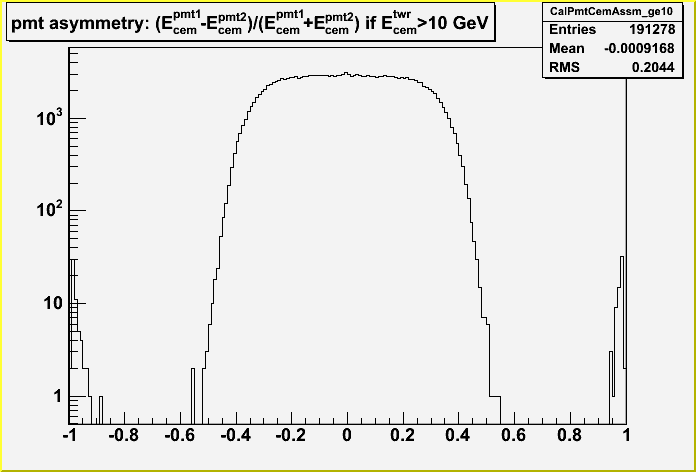
\includegraphics[scale=0.5]{pmt_assym.png}
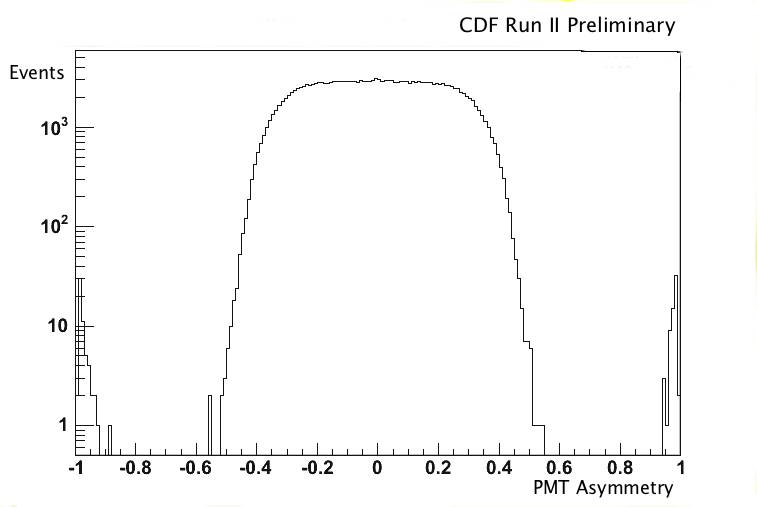
\includegraphics[scale=0.5]{PMT_EM_Asym_twrE_gt_10.jpg}
\caption{PMT Asymmetry.  The clumps at the extremes indicate PMT spikes. These events  lead to fake \met and hence they are thrown out.}
\label{fig-zht}
\end{centering}
\end{figure}


\subsection{\halojets}
This is a non-collision background that overlaps with a real collision. The protons and anti-protons that are not coalesced, upon hitting the beam pipe, create a miniature shower. Only the muons ($\mu$) survive to make it through the beam pipe. These muons (dubbed the beam halo) travel parallel to the beam and interact with the calorimeter, depositing energy to create an EM cluster that passes photon-ID cuts, making it looks like a real photon. Beam halo tend to occupy phi wedges 0 and 23 of the CDF detector.

To identify and reject the beam halo background we use EM timing and topological cuts (see Table~\ref{tab:halocuts}). We estimate the rejection power of the beam halo cuts by selecting events with no reconstructed vertices, which should primarily be from beam halo and cosmic ray backgrounds. Then we look for an in-time (\intimewindow) photon passing tight photon ID cuts and plot the phi-wedge distribution of the photon before and after the halo ID cuts are applied. We count events in phi-wedges 0 and 23 and subtract off the flat component (cosmic) estimated from the phi-wedges 1 through 22.
  
\begin{equation}
 \mathrm{Rejection~Power}= \frac{\mathrm{Events~in~wedges~0,23~after~cuts} - \mathrm{Average~of~wedges~\textrm{1--22}~after~cuts} }{\mathrm{Events~in~wedges~0,23~before~cuts} - \mathrm{Average~of~wedges~\textrm{1--22}~before~cuts} } = 94.8\%
\end{equation}

\noindent The Beam Halo template is made with the following selection criteria. This is normalized to the expected number of events (see Table~\ref{tab:bgsummary}). 

\begin{enumerate}
	\item The run number must be in the good run list.
	\item The event should pass the PHOTON\_25\_ISO, PHOTON\_50 or \mbox{PHOTON\_70} trigger. 
	\item A reconstructed photon with \etg{30} that passes tight photon ID cuts (Table~\ref{tab:tightphotoncuts}). 
	\item Photon should be in-time (\intimewindow)
	\item Photon should be in phi-wedge 0 or 23
	\item Pass beam halo id cuts (Table~\ref{tab:halocuts})
\end{enumerate}

\subsection{\cosmicjets}
This is a case when a cosmic ray (extraterrestrial high energy muon passing through the earth) interacts with the calorimeter. It is a constant background that is independent of the time of the collision. So we use EM timing to make a template for \cosmicjets. We drop the first 400 \pbi of data because it does not have EM timing information to reject this background efficiently.

To estimate the amount of background remaining in the sample, we count events in the time window between \cosmictimewindow and then we extrapolate to the signal window: 

\begin{equation}
\mathrm{Cosmics~left~ in~ the~ sample = \frac{Number~of~events~in~window~\textrm{(30--90~ns)}}{90 - 30} \times (4.8\times2)}
\end{equation}

\noindent The template for this background is made with the following selection rules and it is normalized to the expected number of events (see Table~\ref{tab:bgsummary}).

\begin{enumerate}
	\item The run number must be in the good run list.
	\item The event should pass the PHOTON\_25\_ISO, PHOTON\_50 or \mbox{PHOTON\_70} trigger. 
	\item There should be at least one good class 12 vertex (except in the case of beam halo template).
	\item The $z$-coordinate of the highest-\pt vertex should be within the well-instrumented region, i.e. \mbox{$|z|<60$~cm} (except in the case of beam halo template).
	\item Require one reconstructed photon with \etg{30} that passes tight photon ID cuts (see Table~\ref{tab:tightphotoncuts}). 
	\item Photon should be between \cosmictimewindow
	\item $\geq$1 jets
\end{enumerate}


\subsection{\elejets}
This is a standard model background where an electron fakes a photon because the associated track is not reconstructed. Most of these electrons come from $\w^{\pm} \rightarrow e^{\pm} +\nu$ decay. Less significant contributions come from \z, di-boson, and $\tau$ decays. We use phoenix rejection of photons to remove \elejets events from the sample. Phoenix rejection is about 60\% efficient in rejecting electrons with energies \etg{30}.

To predict the shapes of the remaining \elejets we use an Electroweak Monte Carlo data sample. We identify \phojets events according to the criteria listed below and normalize each background by the luminosity. 

\begin{enumerate}
	\item The run number must be in the good run list.
	\item There should be at least one good class 12 vertex (except in the case of beam halo template).
	\item The $z$-coordinate of the highest-\pt vertex should be within the well-instrumented region, i.e. \mbox{$|z|<60$~cm} (except in the case of beam halo template).
	\item Require one reconstructed photon with \etg{30} that passes tight photon ID cuts (see Table~\ref{tab:tightphotoncuts}).
	\item Reject if phoenix photon 
	\item $\geq$1 jets
\end{enumerate}

\subsection{QCD Background}
This accounts for all the QCD processes that can produce or mimic the \phojets signal, primarily jets faking $\gamma$s. We use $\gamma$ sideband\footnote{Photon passing loose photon ID cuts but failing tight photon ID cuts is termed as sideband photon.} to predict this background. The following selection criteria are used to predict the shape of this background.

\begin{enumerate}
	\item The run number must be in the good run list.
	\item The event should pass the PHOTON\_25\_ISO, PHOTON\_50 or \mbox{PHOTON\_70} trigger. 
	\item There should be at least one good class 12 vertex (except in the case of beam halo template).
	\item The $z$-coordinate of the highest-\pt vertex should be within the well-instrumented region, i.e. \mbox{$|z|<60$~cm} (except in the case of beam halo template).
	\item Require one reconstructed photon with \etg{30} that passes loose photon ID cuts \mbox{(Table~\ref{tab:loosephotoncuts})} and fails tight photon ID cuts (Table \ref{tab:tightphotoncuts}). 
	\item Photon should be in-time, \intimewindow
	\item Not a phoenix photon
	\item Not beam halo
	\item $\geq$1 jets, \etg{15}
\end{enumerate}

\noindent From the CES/CPR weight~\cite{wwwCESCPR}, the fake photon fraction for photons with \etg{30} is determined to be 0.319 $\pm$ 0.001(stat) $\pm$ 0.068(syst)~\cite{wwwCESCPR}. After subtracting cosmic, beam halo and electroweak backgrounds we normalize this background as follows.
\begin{equation}
\mathrm{Normalization = \frac{Total~Number~of~Signal~Events \times 0.319}{Total~Number~of~Sideband~Events}}
\end{equation}

\noindent To fill up the rest, we used \pho Monte Carlo to get the shape of the real photons in the sideband sample. It is normalized in such a way that sum of the sideband fraction and the pure photon fraction to be equal to 100\%.

\section{Systematics Uncertainties}

We have accounted systematic uncertainties of the following. We take the square root of sum of quadratures of all systematic uncertainties to make the error band in the final plots.

\subsection{\cosmicjets}
We choose a smaller time window within the cosmic time window (\cosmictimewindow) and make another prediction of the number of cosmic events left in the sample. The difference of the predictions is taken as the systematic uncertainty.   

\subsection{\elejets}
We take the uncertainty in the Luminosity measurement of the electroweak Monte Carlo data to measure the systematic uncertainty of the electroweak backgrounds, which is ~6\% (This is excluding the uncertainty in the PDFs). We vary the normalization by this uncertainty which gives a different shape for the curve. The difference in the shapes is taken as the systematic uncertainty for electroweak background.

\subsection{\halojets}
Systematic uncertainty for the halos taken to be 50\%  of the bin content as this background is insignificant at this stage of the analysis.


\subsection{Fake and Real Photon Fraction}
We use 100\% of the photon sideband sample to predict the shape of the jet multiplicity. This technique is suitable as the jet multiplicity is independent of the photon \et and hence the photon sideband describes this distribution very well. Other histograms are generated using a combination of photon sideband and the pure photons to get the correct shape. Normalizations for sideband and pure photons are determined a priori using the CES/CPR method~\cite{wwwCESCPR}. The fake photon fraction for photons \etg{30} is calculated to be 0.319 $\pm$0.001 (stat) $\pm$ 0.068 (syst). We apply this fraction to the whole sample, not event by event basis.

There is no correlation between QCD fraction and the pure photon fraction from photon Monte Carlo. The fake photon fraction is used to get the shape and the normalization correctly.

Where we have used the 100\% of the sideband sample, we apply the following prescription to estimate the systematic uncertainty.

\begin{enumerate}
\item Notice that there are four selection ID variables common to both loose photon ID cuts (Table~\ref{tab:loosephotoncuts})  and tight photon ID cuts (Table~\ref{tab:tightphotoncuts}), (Had/Em, Isolation Energy, Track \pt and Track Isolation)
\item Tighten up the loose ID cuts to match the tight photon ID cuts one at a time.
\item Run the sideband sample through the new set of cuts.
\item Normalize the number of events passed back to the sideband sample obtained with the standard set of ID cuts.
\item Divide the variable (histogram) by the corresponding standard sideband variable (histogram).
\item Plot all four histograms obtained by varying the four cuts  on the same histogram for each kinematic variable.
\item Take the maximum variation in each bin to be the systematic uncertainty for that bin.
\end{enumerate}

In the case where we use the mixture of the sideband and the photon Monte Carlo, we vary the mixture within the fake photon fraction's systematic uncertainty to obtain an alternate normalization and hence a different shape of the curve. And take the shift in shape to be the systematics uncertainty due to the fake photon photon fraction.

\subsection{Jet Energy Scale}
We account for jet energy mis-measurement by varying the the jet energy up and down by $\pm \sigma$. We remake the histograms with the shifted jets and take the maximum deviation from the central value as the systematic uncertainty due to jet energy scale and resolution. This is the largest contributor to the final systematic uncertainty.

As for the $\met$ distribution we use the \met resolution model which predicts the contribution to fake \met due to jet energy scale and resolution.


\subsection{EM Energy Scale}
This is to account for the EM energy mis-measurements of the EM objects. We shift the the photon energy by 1\% along with the jet energy scale and take the deviation from the central value as the systematic uncertainty.

\subsection{Statistical Uncertainty}
Statistical uncertainty becomes significant in the high end tail of some variables due to limited statistics in the background expectations. Hence we have incorporated the statistical uncertainty in to the final systematic error.


\begin{figure}
\begin{centering}
\rotatebox{90} {
\includegraphics[scale=0.7]{plot1_pet.pdf} }
\caption{Photon \et for \phoonejet}
\label{fig-p1j_pet}
\end{centering}
\end{figure}

\begin{figure}
\begin{centering}
\rotatebox{90} {
\includegraphics[scale=0.7]{plot2_PhoEt.pdf} }
\caption{Photon \et for \photwojet}
\label{fig-p2j_pet}
\end{centering}
\end{figure}

\begin{figure}
\begin{centering}
\rotatebox{90} {
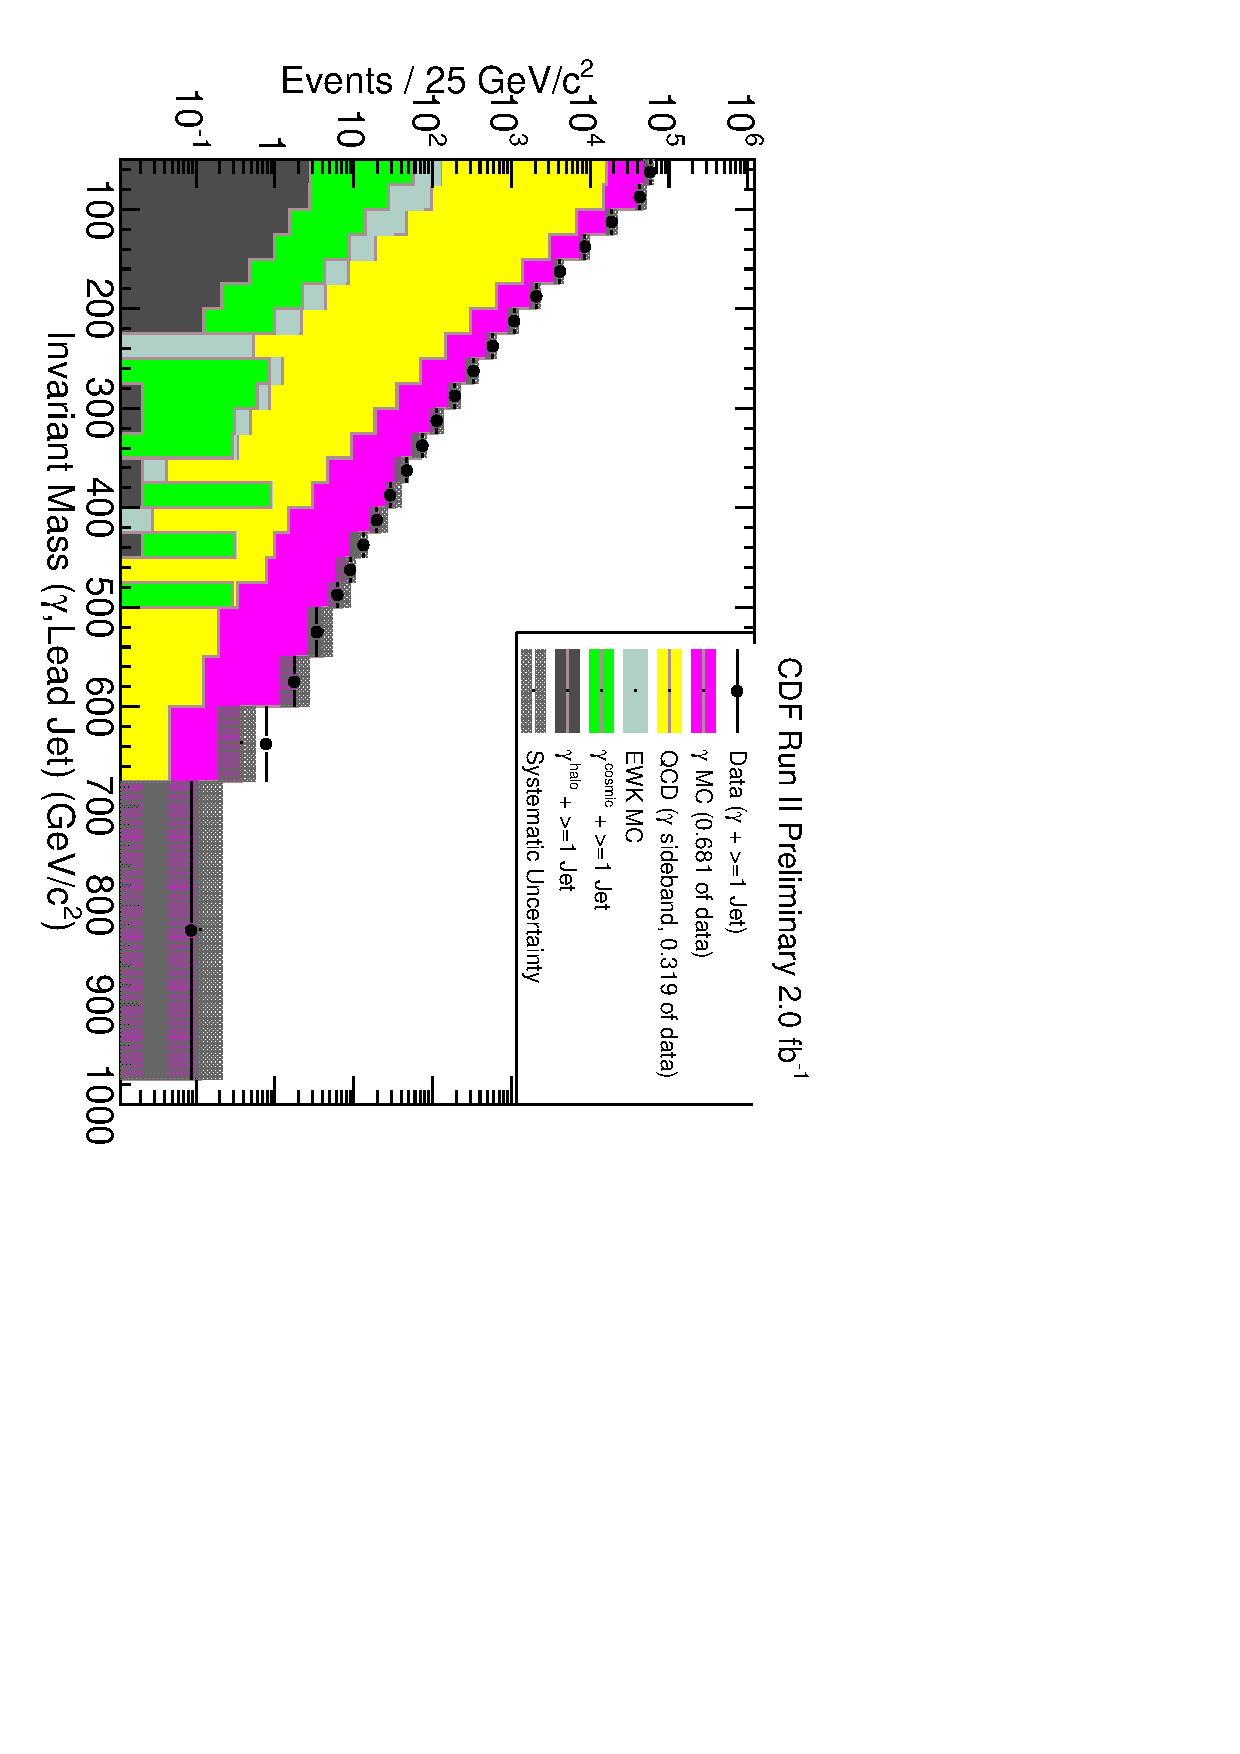
\includegraphics[scale=0.7]{plot1_InvMass.pdf} }
\caption{Invariant Mass of the photon and the lead jet for \phoonejet.}
\label{fig-p1jInvMass}
\end{centering}
\end{figure}



\begin{figure}
\begin{centering}
\rotatebox{90} {
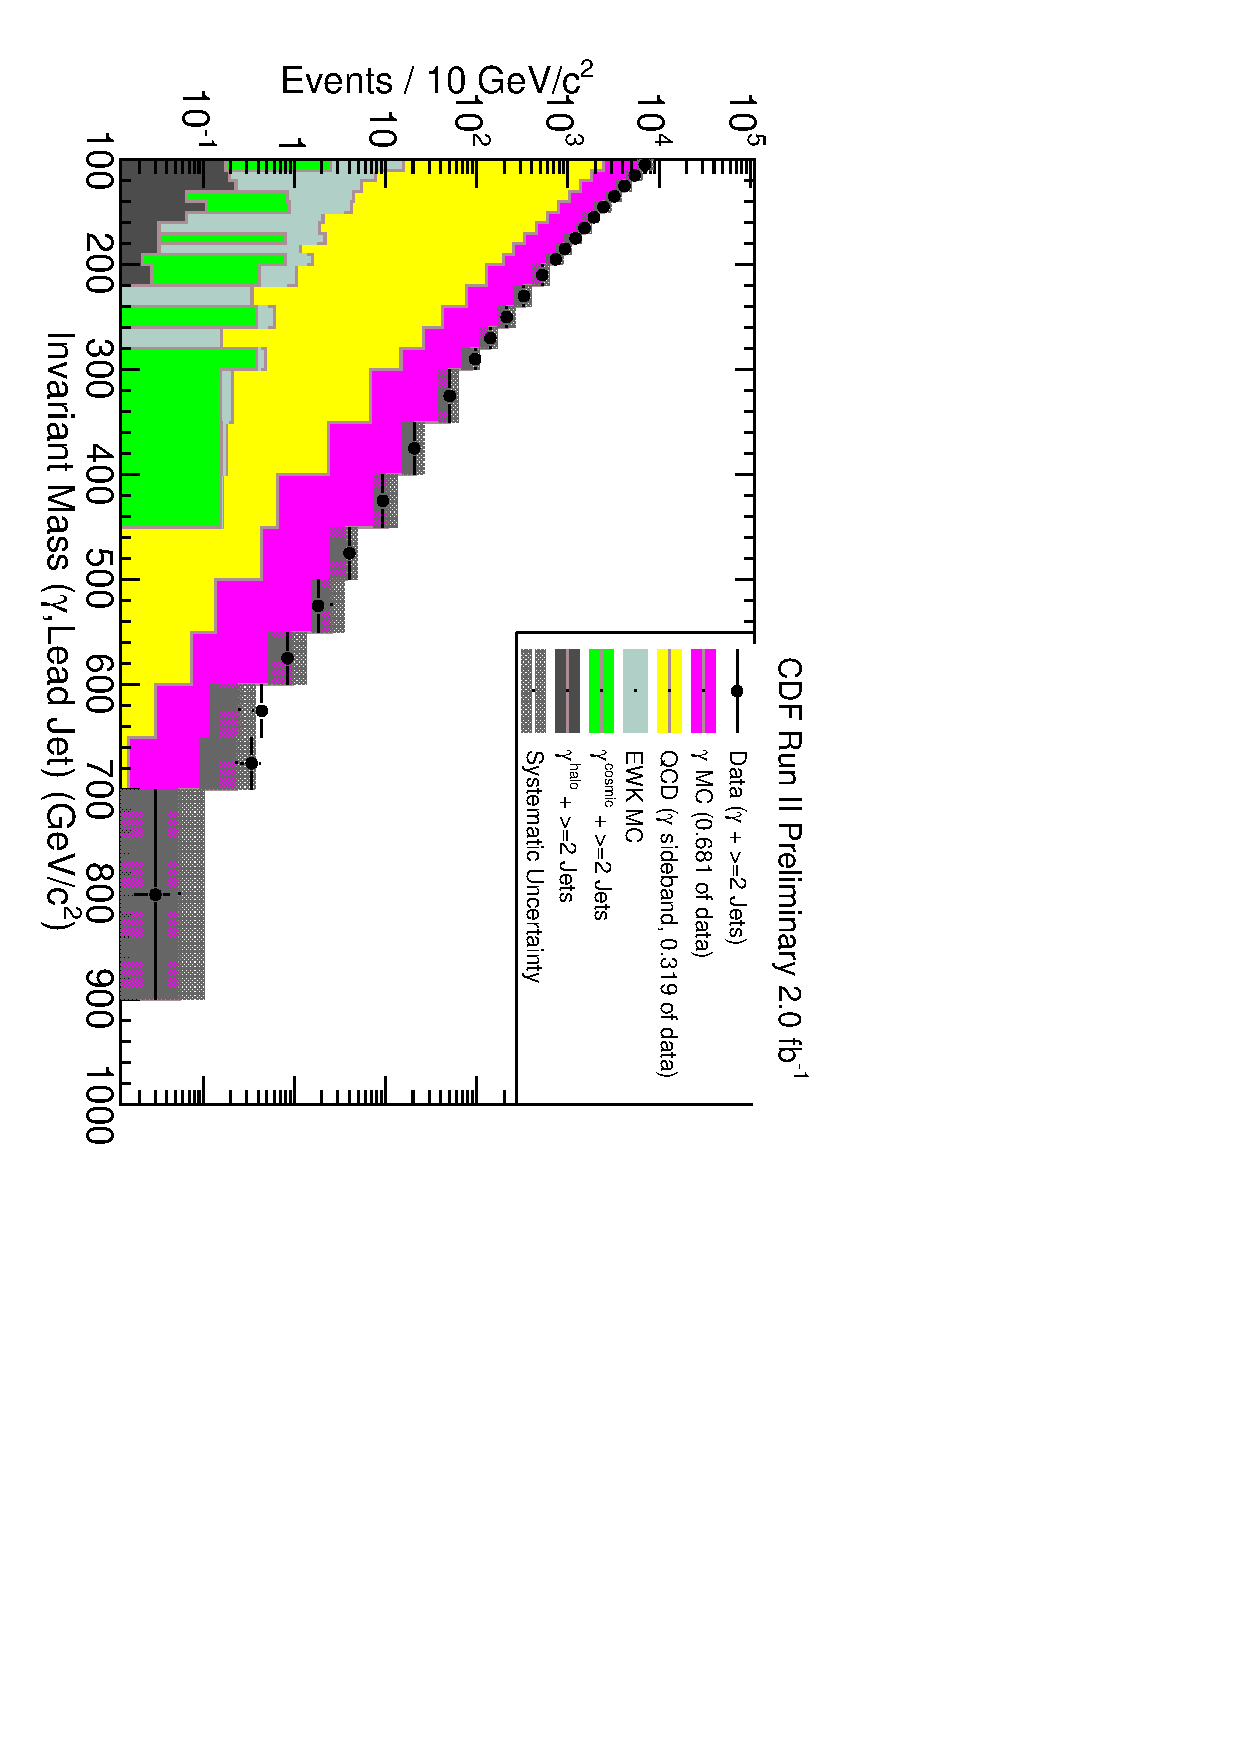
\includegraphics[scale=0.7]{plot2_InvMass.pdf} }
\caption{Invariant Mass of the photon and the two lead jets for \photwojet.}
\label{fig-p2jInvMass}
\end{centering}
\end{figure}

\begin{figure}
\begin{centering}
\rotatebox{90} {
\includegraphics[scale=0.7]{plot2_jetsInvMass.pdf} }
\caption{Invariant Mass of the two leading jets for \photwojet.}
\label{fig-p2jJetsInvMass}
\end{centering}
\end{figure}

\begin{figure}
\begin{centering}
\rotatebox{90} {
\includegraphics[scale=0.7]{plot1_njet.pdf} }
\caption{Jet Multiplicity for \phoonejet}
\label{fig-njet}
\end{centering}
\end{figure}

\begin{figure}
\begin{centering}
\rotatebox{90} {
\includegraphics[scale=0.7]{plot1_ht.pdf} }
\caption{Ht for \phoonejet.}
\label{fig-p1Ht}
\end{centering}
\end{figure}

\begin{figure}
\begin{centering}
\rotatebox{90} {
\includegraphics[scale=0.7]{plot2_Ht.pdf} }
\caption{Ht for \photwojet.}
\label{fig-p2Ht}
\end{centering}
\end{figure}


%\begin{figure}
%\begin{centering}
%\rotatebox{90} {
%\includegraphics[scale=0.7]{plot1_jetsInvMass.pdf} }
%\caption{Invariant Mas of the leading two jets of \photwojets}
%\label{fig-jetsInvMass}
%\end{centering}
%\end{figure}


\section{Summary of Background Estimates}
%%%%%%%%%%%%%%%%%%%% Background Summary %%%%%%%%%%%%%
\begin{table}[h]
\begin{center}
\begin{tabular} {|c|c|c|}
\hline
\bf{Background} & \bf{Expected for $\geq$1Jet} & \bf{Expected for $\geq$2 Jets} \\
\hline
SM Photon  			& 2.6M & 650K \\
\hline
QCD					& 1M & 280K \\
\hline
EWK					& 5362 & 1321 \\
\hline
Cosmic 				& 110 & 7 \\
\hline
Beam Halo			& 9 & $\le$1\\
\hline
PMT Spikes  		  	&  0 	 & 0 \\
\hline
\end{tabular}
\end{center}
\caption{Summary of background estimates. All these are estimated for the full dataset.}
\label{tab:bgsummary}
\end{table}



\section{Acknowledgment}
We like to thank Shin-Shan Eiko Yu providing us with the fake photon fraction and for all the advice. 
Also we want to thank Max Goncharov answering various questions and providing the run dependent EM time corrections. Finally I would like to thank my wife, Vajira, my daughter, Amaya, and my family for their patience and support.

%%%%%%%%%%%%%%%%%%%% Templates Summary %%%%%%%%%%%%%
\begin{table}[hbm]
\begin{center}
\begin{tabular} {|c|c|c|}
\hline
\bf{Background} & \bf{Template Events $\geq$1Jet} & \bf{Template Events $\geq$2 Jets} \\
\hline
SM Photon  			& 231K & 49K \\
\hline
QCD					& 2.1M & 554K \\
\hline
\zee				&  5786 & 1481 \\
\hline
\zmm				& 0 & 0 \\
\hline
\ztt		& 78 & 20\\
\hline
\wen		& 548  & 108\\
\hline
\wmn		& 0  & 0 \\
\hline
\wtn		& 7  & 0 \\
\hline
Cosmic 				& 685 & 43 \\
\hline
Beam Halo			& 35 & 10 \\
\hline
\end{tabular}
\end{center}
\caption{Summary of Number of Events in Background Templates.}
\label{tab:bgteplatesummary}
\end{table}




%%%%%%%%%%%%%% LOOSE PHOTON CUT %%%%%%%%%%%%%
\begin{table}[hbm]
\begin{center}
\begin{tabular} {|c|c|}
\hline
\bf{Variable} 		& \bf{Cut value} 	\\
\hline
detector  		  	& central 	\\
\hline
$\etcorr$ 	& $ >30 $ GeV \\
\hline
CES X and Z fiducial 		& $ |X_{CES}| \leq 21 $ cm \\
				& $ 9 $ cm $ \leq |Z_{CES}| \leq 230 $ cm \\ 
\hline
Had/Em 		&	$ \leq 0.125$ \\
\hline
\isoetcorr in cone 0.4	&  $\leq$ 0.15 $\times \etcorr$ if $\etcorr<$20 GeV\\
					&  $\leq$ 3.0 if \etcorr$>$20 GeV \\
\hline
Track $\pt$ 	& $< 0.25 \times \etcorr$ \\
\hline
Track Iso($0.4$) &	$< 5.0 $ \\
\hline
\end{tabular}
\end{center}
\caption{Loose Photon ID cuts.}
\label{tab:loosephotoncuts}
\end{table}

%%%%%%%%%%% TIGHT PHOTON CUTS %%%%%%%%%%%%%%

\begin{table}[hbm]
\begin{center}
\begin{tabular} {|c|c|}
\hline
\bf{Variable} 		& \bf{Cut value} 	\\
\hline
detector  		  	& central 	\\
\hline
$\etcorr$ 	& $ >30 $ GeV \\
\hline
CES X and Z fiducial 		& $ |X_{CES}| \leq 21 $ cm \\
				& $ 9 $ cm $ \leq |Z_{CES}| \leq 230 $ cm \\ 
\hline
Had/Em 		&	$ \leq 0.125~|| \leq 0.055 + 0.00045 \times \ecorr$ \\
\hline
\isoetcorr in cone 0.4	&  $\leq 0.1 \times \etcorr$ if $\etcorr<20$ GeV\\
					&  $\leq 2.0 + 0.02 \times (\etcorr -20)$ if $\etcorr>20$ GeV \\
\hline
average CES $ \chi^2$ (Strips+Wires)/2	&  $ \leq 20 $ \\
\hline
N tracks in cluster (N3D)	&	$\leq1$ \\
\hline
Track $\pt$ 	& $< 1+0.005 \times \etcorr$ \\
\hline
Track Iso($0.4$) &	$< 2.0 + 0.005 \times \etcorr $ \\
\hline
2\superscript{nd} CES cluster $E \times sin(theta)$ 	&	$ \leq 0.14 \times \etcorr $ if $ \etcorr < 18 $ GeV \\
(both wire and strip E individually)		&	$ \leq 2.4 + 0.01 \times \etcorr $ if $ \etcorr \geq 18 $ GeV \\
\hline
\end{tabular}
\end{center}
\caption{Tight Photon ID cuts.}
\label{tab:tightphotoncuts}
\end{table}



%%%%%%%%%%%%%%% PHOTON-LIKE ELECTRON ID CUTS %%%%%%%%
\begin{table}[hbm]
		\begin{center}
			\begin{tabular} {|c|c|}
				\hline
				\bf{Variable} 		& \bf{Cut value} 	\\
				\hline
				detector  		  	& central 	\\
				\hline
				corrected \et 	& $ >30 $ GeV \\
				\hline
				CES fiduciality 		& $ |X_{CES}| \leq 21 $ cm \\
								& $ 9 $ cm $ \leq |Z_{CES}| \leq 230 $ cm \\ 
				\hline
				average CES $ \chi^2 $	&  $ \leq 20 $ \\
				\hline
				Had/Em 		&	$ \leq 0.055 + 0.00045 \times E $ \\
				\hline
				\isoetcorr in cone 0.4	&	$ \leq 0.1 \times \et $ if $ \et < 20 $ GeV \\
									&	$ \leq 2.0 + 0.02 \times (\et -20) $ if $ \et \geq 20 $ GeV \\
				\hline
				N3D tracks in cluster	&	$= 1,2 $ \\
				\hline
				\eoverp of 1st track	& $0.8 \leq \eoverp \leq 1.2 $ if $ \pt < 50 $ GeV \\
									& no cut if $ \pt \geq 50 $ GeV \\
				\hline
				2nd track $\pt$ if N3D = 2	&	$ \leq 1.0 + 0.005 \times \et $ \\
				\hline
				TrkIso($0.4$) - $\pt$(1st track) &	$ \leq 2.0 + 0.005 \times \et $ \\
				\hline
				\et of 2nd CES			&	$ \leq 0.14 \times \et $ if $ \et < 18 $ GeV \\
				cluster (wire and strip)		&	$ \leq 2.4 + 0.01 \times \et $ if $ \et \geq 18 $ GeV \\
				\hline
				$|\Delta z| = z_{vtx} \-- z_{trk}$	&	$\leq 3$ cm	\\
				\hline

			\end{tabular}
		\end{center}
	\caption{Photon-like electron ID cuts.}
	\label{tab:pecuts}
\end{table}

%%%%%%%%%%%%%%%%%%%% Halo ID cuts %%%%%%%%%%%%%
\begin{table}[hbm]
\begin{center}
\begin{tabular} {|c|c|}
\hline
\bf{Variable} 		& \bf{Cut value} 	\\
\hline
seedWedge  		  	& $>$ 8 	\\
\hline
Nhad 	& $>$ 3\\
\hline
\end{tabular}
\end{center}
\caption{Beam Halo ID cuts. \textit{seedWedge} is defined as number of EM towers (\et$>$0.1 GeV) in the same wedge as $\gamma$ and \textit{Nhad} as the number of plug HAD towers (\et$>$0.1 GeV) in same wedge as $\gamma$.}
\label{tab:halocuts}
\end{table}



%%%%%%%%%%%%%%%%%%%%%%%%%%%%%%%%%%%%%%%%%%%

\begin{thebibliography}{99}

\bibitem{CDF8220} CDF--8220, R. Culbertson {\it et al.}, ``Probability of an Electron Faking an Isolated Prompt Photon in CEM'', May 30, 2006.

\bibitem{CDF9224} CDF--9224, S. Hewamanage {\it et al.}, ``Validation of Photon Sample by Estimating \wen and  \zee  Cross Sections'', March, 2008.

\bibitem{wwwJER} CDF Jet Energy and Resolution Group, ``http://www-cdf.fnal.gov/internal/physics/top/ jets/corrections.html''

\bibitem{wwwCESCPR} CES/CPR method for Photon background from Photon group, ``http://www-cdf.fnal.gov/internal/physics/photon/docs/CesCprMethod.html''


\end{thebibliography}


\end{document}

%%%
